\documentclass[12pt]{article}
\usepackage{amsmath}
\usepackage{amsthm}
\usepackage{amsfonts}
\usepackage{graphicx}
\usepackage{epstopdf}
\usepackage{fontspec}
\usepackage{float}
\usepackage{fancyhdr}
\usepackage{hyperref}
\usepackage{subcaption}
\usepackage{pdfpages}
\usepackage{algpseudocode}
\usepackage{framed}
\usepackage{amssymb}
%\usepackage[round]{natbib}

%\setcitestyle{open={(},close={)}}
%\usepackage{citet}
%\usepackage[toc,page]{appendix}
%\usepackage{libertine}
%\usepackage[libertine]{newtxmath}
\theoremstyle{definition}


\makeatletter
\renewcommand\@biblabel[1]{}
\renewenvironment{thebibliography}[1]
     {\section*{\refname}%
      \@mkboth{\MakeUppercase\refname}{\MakeUppercase\refname}%
      \list{}%
           {\leftmargin0pt
            \@openbib@code
            \usecounter{enumiv}}%
      \sloppy
      \clubpenalty4000
      \@clubpenalty \clubpenalty
      \widowpenalty4000%
      \sfcode`\.\@m}
     {\def\@noitemerr
       {\@latex@warning{Empty `thebibliography' environment}}%
      \endlist}
\makeatother


\newtheorem{riskmeasure}{Definition}
\newtheorem{theorem}{Theorem}
\newtheorem{lemma}{Lemma}
\allowdisplaybreaks
%\setmainfont{Calibri}
%\pagestyle{fancy}
\fancyhf{}
%\lhead{Audit Services | Quantitative Analysis}
%\rhead{ BB\&T \thepage}

\DeclareMathOperator*{\Max}{Max}
\DeclareMathOperator*{\Min}{Min}
\setlength{\parindent}{0cm}



\begin{document}

\title{Correlated latent variables in m dimensions}
\date{}
\author{Daniel H. Stahl\\Internal Auditor, BB\&T
        \\dstahl@bbandt.com}

\maketitle
Word Count: 3369
\\
\\
Figures and Tables: 8
\\
\\
Acknowledgments: The author reports no conflicts of interest.  The author alone is responsible for the content and writing of the paper.
\newpage
 
\section{Model Description}
The model setup is similar to the setup in Stahl (2015).  The main features of this model are independent defaults conditional on latent factors, mutually independent losses given default, and a semi-endogenous risk of a liquidity event.  The model in this paper distinguishes itself from Stahl (2015) in three important points.  First, the process that drives correlation is now an \(m\) dimensional process.  These processes represent the exposure of the assets to various factors.  For instance, a loan to a business in rural New Mexico or the south east may have more risk than a a loan to a business in Texas or San Francisco.  A loan to a tech business in Texas may have different risks than a loan to an energy business in Texas.  Each of these risks (geographic, industry, or otherwise) can be captured by a distinct dimension of the process.  
\\
\\
The second key difference is that these process are jointly normally distributed: in particular, by a multi-dimensional Ornstein-Uhlenbeck process.  This assumption is important for several reasons.  Normally distributed processes lend themselves to analytic tractability including the ability to easily implement a correlation structure across the factors.  The normality also allows for relatively simple transition from a CAPM and Merton type framework.  While there are many benefits to using Gaussian processes, such processes have the unfortunate property of having the positive probability of negative values.  As the probabilities of default are affine functions of the processes, this feature of Gaussian models allows for negative probabilities of default.  However, the probability of negative values need not be large; and since the integral of the process is used for determining the factors affecting the default probability the probability of having negative probabilities becomes essentially negligible.  
\\
\\
The third difference is that the risk of a liquidity crisis is an affine function of the assets' exposures.  Modeling liquidity exposure in this manner allows liquidity risk to be charged at the loan level and provides a relatively simple method to quantify and aggregate liquidity risk in terms of common funding practices like FHLB and FRB pledging.  However, this flexible modeling comes at the price of losing the linearity of the portfolio in the sense of Tasche (2008).  The main drawback is that Euler contributions no longer are the ``correct'' method for aggregating risk as the sum of the risk contributions no longer equal the entire portfolio risk.  While concerning, this drawback is overcome by using some sensible and straightforward criteria in section \ref{appXTLambda}.

This paper introduces the model and then uses examples to demonstrate how such a model may be used in an actual loan portfolio.  
\section{General framework}
In Stahl (2015), the goal was to find an analytical expression for the characteristic function of the portfolio loss so that numerical inversion could be efficiently applied to recover the density function of the loss distribution.  This paper adopts a nearly identical framework: a portfolio \(X_t=\sum_j X_t ^ j\) contains \(n\) assets \(X_t ^ j\) with mutually independent exposures \(l_j\).  Each asset has a probability of default.  In Stahl (2015) the probability of default was driven by a single Brownian motion; in this paper this is extended so that the instantaneous probability of default for asset \(j\) is an affine function of an \(m\) dimensional mean-reverting Levy process \(L_t\) with long run expected value equal to a vector of ones.  Letting the filtration generated by the Levy process be denoted \(\mathcal{F}_t\) and the filtration of the entire process \(X_t\) be denoted \(\mathcal{G}_t\), the probability of default for asset \(X_t ^ j\) conditioned on \(\mathcal{G}_t\) over the interval \([t, T]\) is \(\left(w_j ^ T \int_t ^ T L_s ds  \right) p_j\) where \(w_j\) is a constant normal vector, \(p_j\) is a constant, and a superscript \(T\) denotes the transpose.  Since the instantaneous default probability is \(w_j ^T L_t p_j dt\) which has long run expected value \(p_j dt\),  it is convenient to think of \(p_j\) as the long run instantaneous probability per unit time.  Following the logic in (Stahl 2015), the approximate characteristic function of \(X_T-X_t\) conditioned on \(\mathcal{G}_t\) is 
\begin{equation}
\phi_{X_T}(u)=\mathbb{E}\left[e^{\sum_j \left(w_j ^T \int_t ^ T L_s  ds \right) p_j (\phi_j(u)-1)} |\mathcal{G}_t\right]
\end{equation}
Where \(\phi_j(u)\) is the characteristic function of \(l_j\).  \(\phi_{X_T}(u)\) can be written as 

\begin{equation}
\(\phi_{X_T}(u)\)=\mathbb{E}\left[e^{\sum_k  \int_t ^ T L_s  ds \sum_j w_{j, k}  p_j (\phi_j(u)-1)} |\mathcal{G}_t\right]
\end{equation}
\begin{equation} \label{CharFY}
=\mathbb{E}\left[e^{z^T \int_t ^ T L_s  ds } |\mathcal{G}_t\right]=\mathbb{E}\left[e^{z^T (Y_T-Y_t) } |\mathcal{G}_t\right]
\end{equation}
Where \(z=\sum_j w_{j, k}  p_j (\phi_j(u)-1),\,\,k \in [1,...,m]\) and \(Y_t=\int_0 ^t L_s ds\).  But this is just the moment generating function of \(Y_t\).  As long as the moment generating function of \(Y_t\) has an analytical expression, the characteristic function has a closed form solution and can be efficiently inverted.  Examples of \(Y_t\) that satisfy this constraint in a diffusion setting can be found in Duffie et. al. (2000) while examples of \(Y_t\) that are the more general Levy process is found in  Filipovic (2001).  As far as the author knows, there is no more general formulation of the basic loss distribution.  Within the framework the problem reduces to finding suitable processes \(Y_t\).  

\section{Latent Process}
For this paper, the process \(L_t\) is assumed to solve the following stochastic differential equation (SDE):

\[dL_t={A} (\mathbf{1}-{L_t}) dt +{\Sigma}d {W_t}\] 
 \({A}\) is an \(m x m\) diagonal matrix with \({A}_{i, i}>0, \,\, i = 1, ..., m\), \(\mathbf{1}\) is an \(m x 1\) vector of ones, \({\Sigma}\) is an \(m x m\) matrix satisfying \({\Sigma}{\Sigma}^T={\Omega}\) where \({\Omega}\) is positive semi-definite, and \(d{W_t}\) are independent increments of an \(m x 1\) Brownian motion.  \({\Omega}_{i, j}=\sigma_i \sigma_j \rho_{i, j},\,\,  i,\,j = 1, ...,m\) where \(\sigma_i>0\), \(\rho_{i, j} \in [-1, 1]\), and \(\rho_{i, i}=1\).

\subsection{Solution to the SDE}

By Ito's Lemma, 
\begin{equation} d\left(e^{{A}t}{L_t}\right)={A}e^{{A}t}{L_t}dt+e^{{A}t}{A} (\mathbf{1}-{L_t}) dt +e^{{A}t}{\Sigma}d {W_t} \end{equation}
The matrix exponential is, as usual, defined as \(e^{{A}}=\sum_{j=0} ^ \infty \frac{{A}^j }{j!}\).  Since \({A}\) is diagonal, this simplifies to \(\text{diag}\left(e^{A_{ii}}\right)\).
\begin{equation} d\left(e^{{A}t}{L_t}\right)=e^{{A}t}{A} \mathbf{1} dt +e^{{A}t}{\Sigma}d {W_t} \end{equation}
Integrating,
\begin{equation} e^{{A}T}{L_T}=L_0+e^{AT} \mathbf{1}-\mathbf{1}+\int_0 ^ T e^{{A}t} {\Sigma}d {W_t} \end{equation}
Solving for \(L_T\),
\begin{equation} \label{solutionL} {L_T}=e^{-AT}(L_0-\mathbf{1})+ \mathbf{1}+e^{-AT}\int_0 ^ T e^{{A}t} {\Sigma}d {W_t} \end{equation}
%\begin{equation}L_T=e^{-AT}L_0+\left[\begin{array}{c}1- e^{-{A}_{1, 1}T}\\ \vdots \\1-e^{-{A}_{m, m}T} \end{array} \right]+e^{-AT}\int_0 ^ T e^{{A}t} {\Sigma}d {W_t} %\end{equation}
As this equation is deterministic in volatility, the distribution of \(L_t\) is normal.  

\subsection{Moments of \(Y_T\)} 

Recall that the probability of default is an affine function of \(Y_T=\int_0^T L_t dt\).  Since \(L_t\) is Gaussian, the integral of \(L_t\) is also Gaussian.  The moment generating function of a Gaussian random variable with mean \(\mu\) and variance \(\sigma^2\) is the following (reference any statistics text book):

\begin{equation}\phi_{\mathrm{Gaussian}}(u)=\label{GaussianMGF} e^{u\mu +\frac{u^2\sigma^2}{2}} \end{equation}

Thus equation (\ref{CharFY}) reduces to the computation of the expectation and variance of \(z^T Y_T\).  The expectation and variance the following:
\begin{equation} \mathbb{E}[z^T Y_T]=\mu(z)=\sum_{i=1} ^ m z_i T+\frac{z_i}{A_{i,i}}\left(1-e^{-{A}_{i, i}T}\right)(L_0^ i-\mathbf{1})\end{equation}

\begin{multline}\label{varianceY} \mathbb{V}(z^T Y_T)=\sigma^2(z)=\\ \sum_i \sum_j \rho_{i,j} \frac{ z_i z_j \sigma_i \sigma_j}{A_{i,i} A_{j,j}} \left(T-\frac{1-e^{-A_{i,i}T}}{A_{i,i}}-\frac{1-e^{-A_{j,j}T}}{A_{j,j}}+\frac{1-e^{-(A_{i,i}A_{j,j})T}}{A_{i,i}+A_{j,j}}\right) \end{multline}

See appendix A (REF) for a full derivation.

\section{Liquidity Risk} \label{riskContributions}
In Stahl (2015) liquidity risk is modeled by a constant exposure (fixing time) and a probability of a ``crisis'' that is linear in the dollar credit loss.  This allowed the characteristic function of the portfolio loss to retain the same analytical form.  In this paper this concept is generalized further so that the exposure in the case of a liquidity ``crisis'' is an affine function of the individual asset balances at time \(t\).  Using this method retains the analytical characteristic function but also allows liquidity capital to be pushed down to individual loans.  In the case of a liquidity event (which increases in probability as credit losses mount), loans typically must be liquidated at large discounts to par to meet obligations.  The probability of this event occurring (at time \(T\)) is \(q X_T\) where \(X_T\) is the realization of the losses within the portfolio.  In Stahl (2015) the exposure was a fixed constant \(\lambda\).  

\subsection{Characteristic function and Loss distribution Moments}
From Stahl (2015), equation (\ref{CharFY}), and equation (\ref{GaussianMGF}), the characteristic function including liquidity risk is

\begin{equation} \label{finalCH}
\phi_{X_T ^ \lambda}=e^{\mu(z^\lambda)+\frac{\sigma^2(z^\lambda)}{2} }
\end{equation}
Where \(z^\lambda=\sum_j w_{j, k}  p_j (\phi_j(u^\lambda )-1)\) and \(u^\lambda=u-iq\left(e^{ui\lambda}-1\right)\).  The moments for the loss distribution are
\begin{equation} \mathbb{E}[X_T]=\mu(d) \end{equation}
Where \(d\) is the vector  \(d=\frac{1}{i}\sum_j p_j \phi_j'(0) w_{j, k}\).
\begin{equation}\mathbb{V}(X_T)=\mu(d ^2)+\sigma^2(d) \end{equation}
Where \(d ^2\) is the vector \(d^2=-\sum_j p_j\phi_j''(0) w_{j, k}\).
\begin{equation} \mathbb{E}[X_T ^ \lambda]=\mathbb{E}[X_T](1+q\lambda) \end{equation}
\begin{equation} \mathbb{V}(X_T ^ \lambda)=\mathbb{V}(X_T)(1+q\lambda)^2+\mathbb{E}[X_T]q\lambda^2\end{equation}
\subsection{Risk Contributions}

The departure from Stahl (2015) is that the exposure is decomposed as \(\lambda=\lambda_0+\sum_j r_j b_j\) where \(b_j\) is the balance of the asset.  The \(r_j\) can be thought of as the liquidity equivalent to the ``loss given default'' from credit risk vernacular.  \(r_j\) is affected by the market for the asset.  If \(X_t ^ j\) is a conforming mortgage it will likely have a low \(r_j\) since there tends to be a deep and liquid secondary market for conforming mortgages.  Likewise loans pledged to the Federal Home Loan Bank or the Federal Reserve as part of a contingency funding plan will have a lower \(r_j\) since they already have a buyer.  The random variable describing the portfolio loss is the following:
\begin{equation}X_T ^ \lambda=\sum_j X_T ^ j+q\left(\sum_j X_T ^ j\right)\left(\lambda_0+\sum_j b_j r_j\right)\end{equation}
For the computation of the entire portfolio distribution there is no difference how \(\lambda\) is decomposed so long as \(\lambda\) stays fixed.  However, decomposing \(\lambda\) makes a tremendous difference when allocating risk to sub-portfolios.  
\\
\\
Denote the whole portfolio risk by \(\rho(S)\) where \(S: \Omega \to \mathbb{R} ^ n \) is a random variable representing a risky portfolio.  \(\rho\) is typically a statistic similar to Value at Risk (VaR) or expected shortfall (Artzner 1999).  The portfolio \(\rho\) can be found for \(X_T ^ \lambda\) by inverting the characteristic function (\ref{finalCH}) to recover the density as described in Stahl (2015). 
\\
\\
 Pricing, optimization, and performance monitoring requires the allocation of risk capital to any subset of the portfolio.  There are a number of methods for allocating this risk to the portfolio.  A method favored by a number of authors (Tasche 2008, LIST MORE) is the Euler allocation.  

\begin{riskmeasure}
The \emph{Euler allocation} for risk to a sub-portfolio, denoted \(\rho_B(S)\), is as follows:
 \[ \rho_B(S)=\frac{d\rho(S+hB)}{dh} \bigg|_{h=0}\]
\end{riskmeasure}


\begin{theorem}[Euler]
If \(\rho\) is homogeneous of degree one, then for all \(B_i \subset S\) satisfying  \(B_i \cap B_j =\varnothing\), 
\begin{equation}
\sum_i \rho_{B_i} (S) =\rho (S)
\end{equation}
\end{theorem}

A particularly simple form for \(\rho_{B_i}\) is when \(\rho(S)=\mu(S)+c\sigma(S)\).  It is typical to let \(c\) be the value that sets \(\rho(S)\) equal to some portfolio level risk metric such as VaR.  The risk contribution for \(\mu(S)+c\sigma(S)\) is 
\begin{equation}
\rho_{B_i}=\mu(B_i)+c\frac{\mathrm{cov}(B_i,\,S)}{\sigma(S)}
\end{equation}
\subsection{Application to \(X_T\)}
In the case of \(X_T\), it is useful to introduce the following ``partial'' variance function 
\begin{multline} \sigma^2(z^1, z^2)=\\ \sum_i \sum_j \rho_{i,j} \frac{ z_i^1 z_j^2 \sigma_i \sigma_j}{A_{i,i} A_{j,j}} \left(T-\frac{1-e^{-A_{i,i}T}}{A_{i,i}}-\frac{1-e^{-A_{j,j}T}}{A_{j,j}}+\frac{1-e^{-(A_{i,i}+A_{j,j})T}}{A_{i,i}+A_{j,j}}\right) \end{multline}
This function is related to \ref{varianceY} by \(\sigma^2(z, z)=\sigma^2(z)\).  Using this function, the risk contribution is as follows (see appendix for full derivation):
\begin{equation}
%\sigma_Y^2 p_k \mu_{l_k} \sum_j p_j \mu_{l_j}-\mu_Y p_k \phi_{l_k} ''(0) 
\frac{1}{i}p_j \phi_j '(0) \left(\mu (w_j)+ \sigma^2(w_j, d)\right)-  p_j\phi''(0)  \mu(w_j)
\end{equation}
%Where \(d\) is the vector \(d=\sum_j p_j l_j w_{j, k}\).
\subsection{Application to \(X_T ^ \lambda\)} \label{appXTLambda}
While the Euler allocation principal is useful for \(X_T\),  it does not apply for \(X_T ^ \lambda\).   \(X_T ^\lambda\) is not ``linear'' with respect to the individual assets in the following sense:
\[\nexists f:\mathbb{R} \to \mathbb{R} \mid hX_T^\lambda= h f\left(\sum_j X_T ^ j\right)\]
In fact, 
\[ hX_T^\lambda=h\sum_j X_T ^ j+qh\left(\sum_j X_T ^ j\right)\left(\lambda_0+h\sum_j b_j r_j\right) \]

This equation is non-linear in \(h\) and so the homogeneity constraint on \(\rho\) will not hold.  However, it is still possible to allocate risk to each asset within the portfolio using simple and intuitive criteria.  To develop these criteria, it is important to note that the homogeneity constraint does still hold if \(r_j=0\,\forall j\).  Indeed, the risk contribution in this case is the following:
\begin{multline} \label{liquidRiskC}
 \rho_j(X_T ^ \lambda)=\frac{1}{i}p_j \phi_j '(0)\mu(w_j) \left(1+q\lambda_0  + q \lambda_0 ^2  \right) \\+\left(\frac{1}{i}p_j \phi_j '(0) \sigma^2(w_j, d)-p_j\phi''(0)   \mu(w_j) \right)(1+q \lambda_0)^2 
\end{multline}
 
 The availability of the homogeneous risk measure for the case where \(r_j=0\) helps inform the criteria for risk contributions in the case without a homogeneous risk function.  
\begin{enumerate}
\item If \(r_j=0\), then \(X_j\) must not increase the impact of a liquidity event

\item  If \(r_j=0\,\forall j\), risk contributions must equal equation (\ref{liquidRiskC})
\item\( \sum_{j} \rho_i =\rho \)
\end{enumerate}

Using these criteria, the covariance risk contributions to the portfolio variance is as follows:
%\begin{multline} \label{liquidityRiskContributions}
%\rho_j(X_T ^ \lambda)=p_j l_j \mu(w_j)(1+q\lambda_0)+r_j b_j q \mathbb{E}[X_T]\\+\left(p_j l_j ^2  \mu(w_j)+p_j  l_j \sigma^2(w_j, d) \right)(1+q \lambda_0)^2 
%+p_j l_j q \lambda_0 ^2 \mu(w_j) \\
%+2 r_j b_j q \mathbb{V}(X_T)+r_j b_j q^2 \mathbb{V}(X_T)(\lambda+\lambda_0)+r_j b_j (\lambda_0+\lambda)q \mathbb{E}[X_T]
%\end{multline}

\begin{multline} \label{liquidityRiskContributions}
\rho_j(X_T ^ \lambda)=\frac{1}{i}p_j \phi_j '(0)\mu(w_j) \left(1+q\lambda_0  + q \lambda_0 ^2  \right)+r_j b_j q \mathbb{E}[X_T] \\+\left(\frac{1}{i}p_j \phi_j '(0) \sigma^2(w_j, d)-p_j\phi''(0)   \mu(w_j) \right)(1+q \lambda_0)^2 \\
+2 r_j b_j q \mathbb{V}(X_T)+r_j b_j q^2 \mathbb{V}(X_T)(\lambda+\lambda_0)+r_j b_j (\lambda_0+\lambda)q \mathbb{E}[X_T]
\end{multline}




%The appendices in Stahl (2015) provide the solution to the covariance of an asset with the portfolio within the current modeling framework.  


%\begin{riskmeasure}
%A random variable \(S\) has \emph{linear risk} if for all \(B_i \subset S\) satisfying  \(B_i \cap B_j =\varnothing\), 
%\[\bigcup_i h B_j =hS\]
%\end{riskmeasure}




%The condition that \(\rho(S)\) be homogeneous is relatively benign in: most popular risk measures like VaR, expected shortfall, and standard deviation are all homogeneous of degree one (Tasche 2008 TRY TO CITE SOMEONE ELSE EHERE).  However the requirement that \(S\) have \emph{linear risk} is not met for \(X_T ^ \lambda\). 





%The total risk can be found by inverting the characteristic function to recover the density and finding the Value at Risk (VaR) or some similar statistic. 

%Tasche (2008) provides an axiomatic and robust framework for allocating capital to entities within a portfolio.  Given a risk measure \(\rho: \mathbb{R} \to \mathbb{R}\) that satisfies \(\rho(hS)=h^\tau \rho(S), \,\tau,\,h>0\)) for a random variable \(S\), the Euler allocation principal allows the capital allocated to a subset of the portfolio to add up to the total capital of the portfolio.  A particularly tractable risk measure for dividing capital is the ``covariance'' approach which allocates capital based on the covariance of an individual asset with the entire portfolio.  




\section{Worked Example}
\subsection{Overview}

The goal in this section is to apply the framework of section \ref{riskContributions} to a simple portfolio.  The framework can be summarized as follows:
\begin{enumerate}
\item Find the portfolio risk measure \(\rho(X_T ^\lambda)\) (eg, VaR)
\item Find \(c\) such that \(\mathbb{E}\left[X_T ^ \lambda\right]+c \sqrt{\mathbb{V}(X_T ^ \lambda)}=\rho(X_T ^ \lambda)\)
\item Allocate risk to each asset via equation (\ref{liquidityRiskContributions})
\end{enumerate}

\subsection{Example Portfolio}
Consider \(5\) loans with the following features:

\begin{table}[H]
\centering
\begin{tabular}{cccccc}
&\(X_T^1\) & \(X_T^2\)& \(X_T^3\)& \(X_T^4\)& \(X_T^5\) \\
\hline
p& .005 & .01& .015& .02& .025 \\
l & 987 &2104 & 1264 & 576 &377 \\
r & .13 & .15 & .18 & .14 & .78 \\
\end{tabular}
\end{table}

For simplicity in this example \(b_j=l_j\, \forall j\) and \(l_j\) are constants.  Each loan has exposure to 3 risk drivers \(Y\) which is parameterized as follows:

\begin{equation}
{A}=\left[ \begin{array}{ccc} .3 & 0& 0 \\ 0 & .2 & 0 \\ 0 & 0 & .1 \end{array} \right]
\end{equation}

\begin{equation}
{\Sigma}=\left[\begin{array}{ccc} .2 & 0 & 0 \\ .02 & .09797959 & 0 \\ -.09 & .07960842 & .2748863 \end{array}\right]
\end{equation}

\begin{equation}
{L}_0=\left[ \begin{array}{c}1.1\\.9\\.7 \end{array} \right]
\end{equation}

Where the matrix \({\Sigma}\) is constructed from the correlation matrix
\begin{equation}
{\rho}=\left[\begin{array}{ccc} 1 & .2 & -.3 \\ .2 & 1 & .1 \\ -.3 & .1 & 1 \end{array}\right]
\end{equation}

and the matrix of volatilities
\begin{equation}{\sigma}=
\left[\begin{array}{ccc} .2 & 0 & 0\\ 0 & .1 & 0 \\0 & 0 & .3 \end{array}\right]
\end{equation}

such that 
\[{\Omega}={\sigma}{\rho} {\sigma}\]

Figures \ref{fig1} and \ref{fig2} shows sample paths of the process \({L}\) and \({Y}\).
\\
\\
The exposure that each asset has to each of the three risk drivers is represented by the following matrix:

\begin{equation}
{w}=\left[ \begin{array}{ccc}
 .17 & .44 & .39 \\
.04 & .47 & .49 \\
.02 & .87 & .11 \\
.41 & .19 & .40 \\
.52 & .31 &.17 
\end{array}\right]
\end{equation}

The instantaneous default probability is thus obtained by the multiplication \({p} ^T {w}{L}_t dt \).  The plots of a sample path for each asset's probability of default is given in \ref{fig3} and \ref{fig4}.  



\begin{figure}[htb]
\begin{framed}
Sample paths of \({L}\) and \({Y}=\int {L} dt\) \newline
\begin{minipage}[t]{.48\textwidth}
\centering
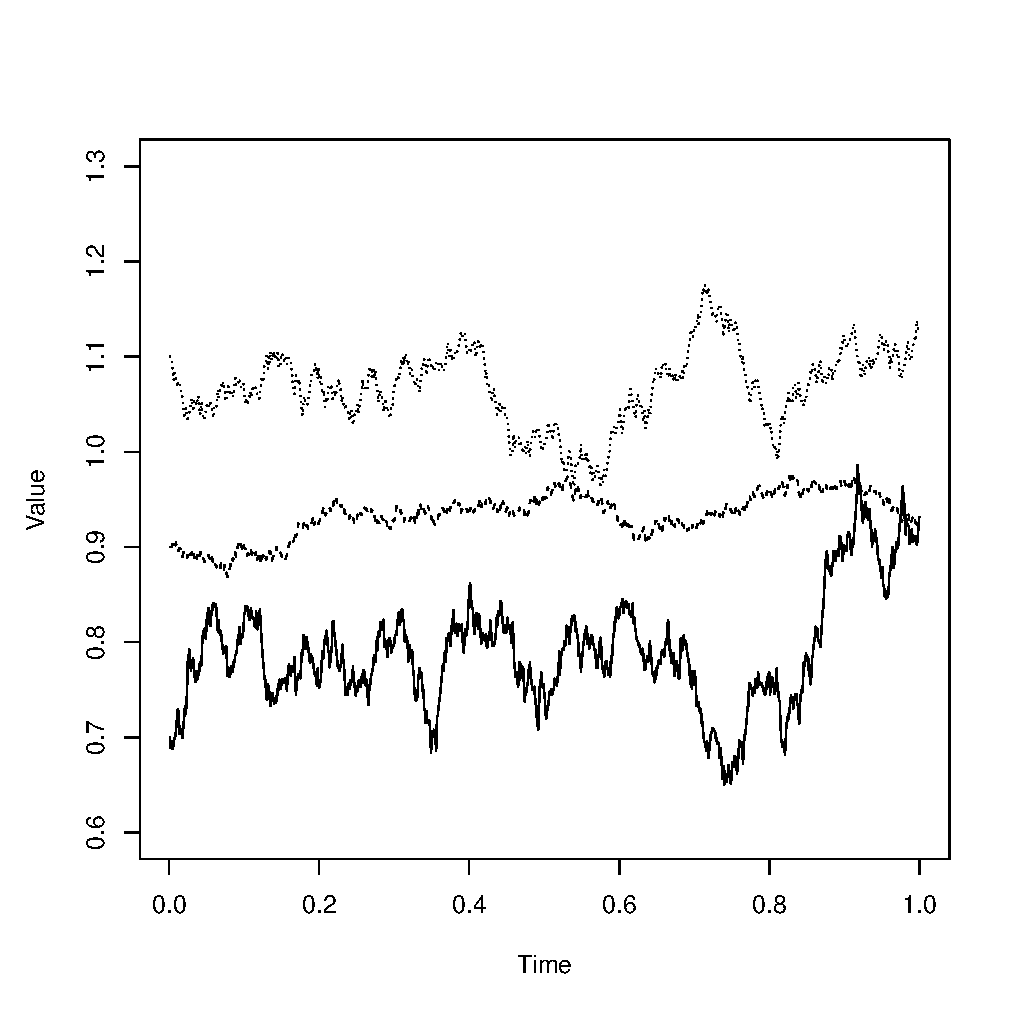
\includegraphics[width=1\textwidth]{StahlPaper2Z}
\caption{ \label{fig1}}
\end{minipage}\hfill
\begin{minipage}[t]{.48\textwidth}
\centering
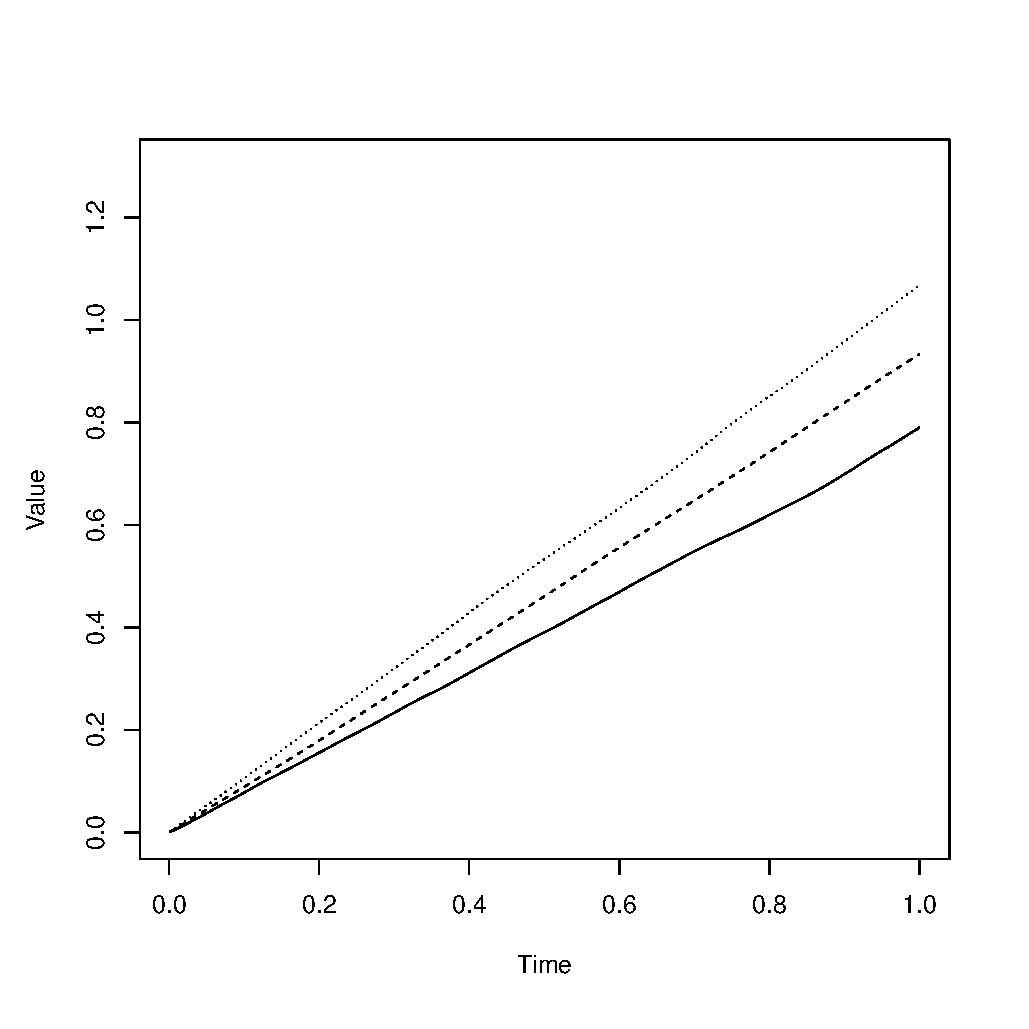
\includegraphics[width=1\textwidth]{StahlPaper2Y}
\caption{ \label{fig2}}
\end{minipage}\hfill
\end{framed}
\end{figure}


\begin{figure}[htb]
\begin{framed}
Sample paths of the probability of default\newline
\begin{minipage}[t]{.48\textwidth}
\centering
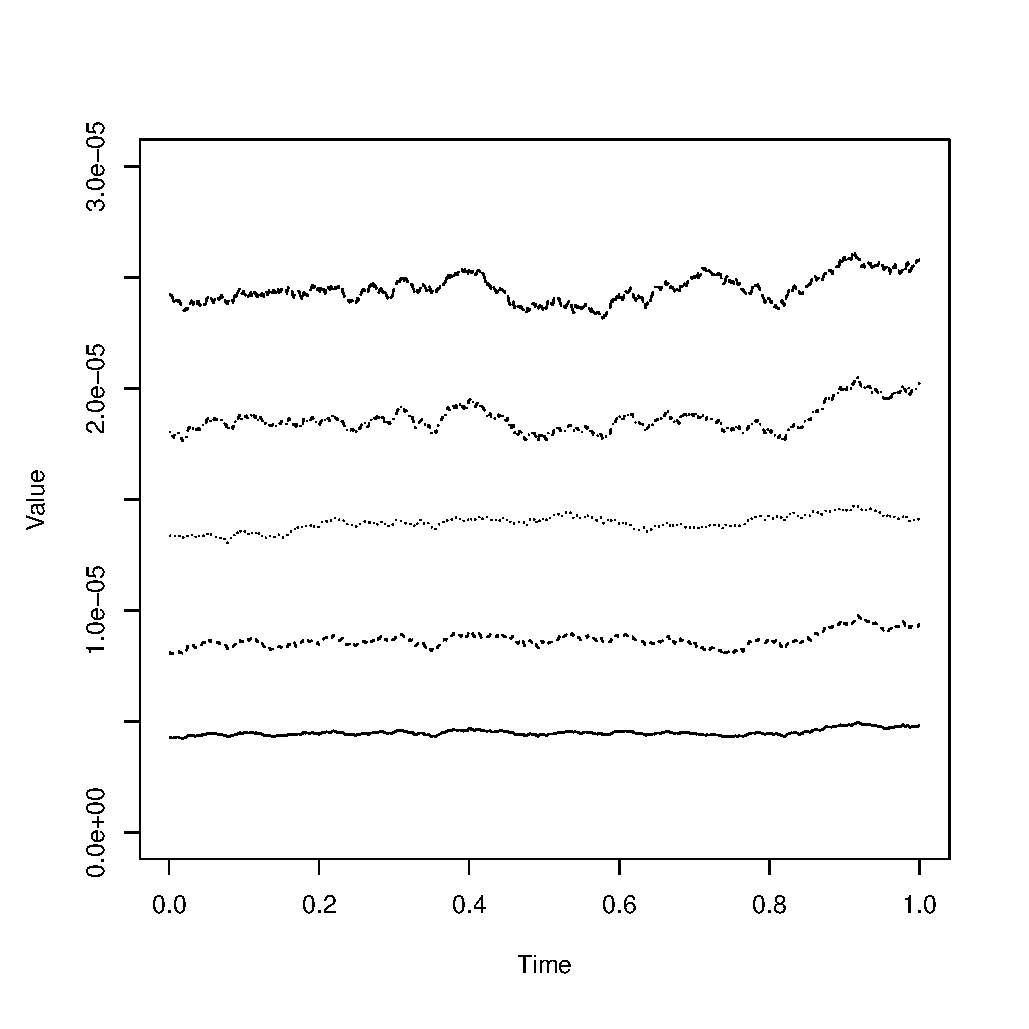
\includegraphics[width=1\textwidth]{StahlPaper2P}
\caption{Instantaneous probability of default \label{fig3}}
\end{minipage}\hfill
\begin{minipage}[t]{.48\textwidth}
\centering
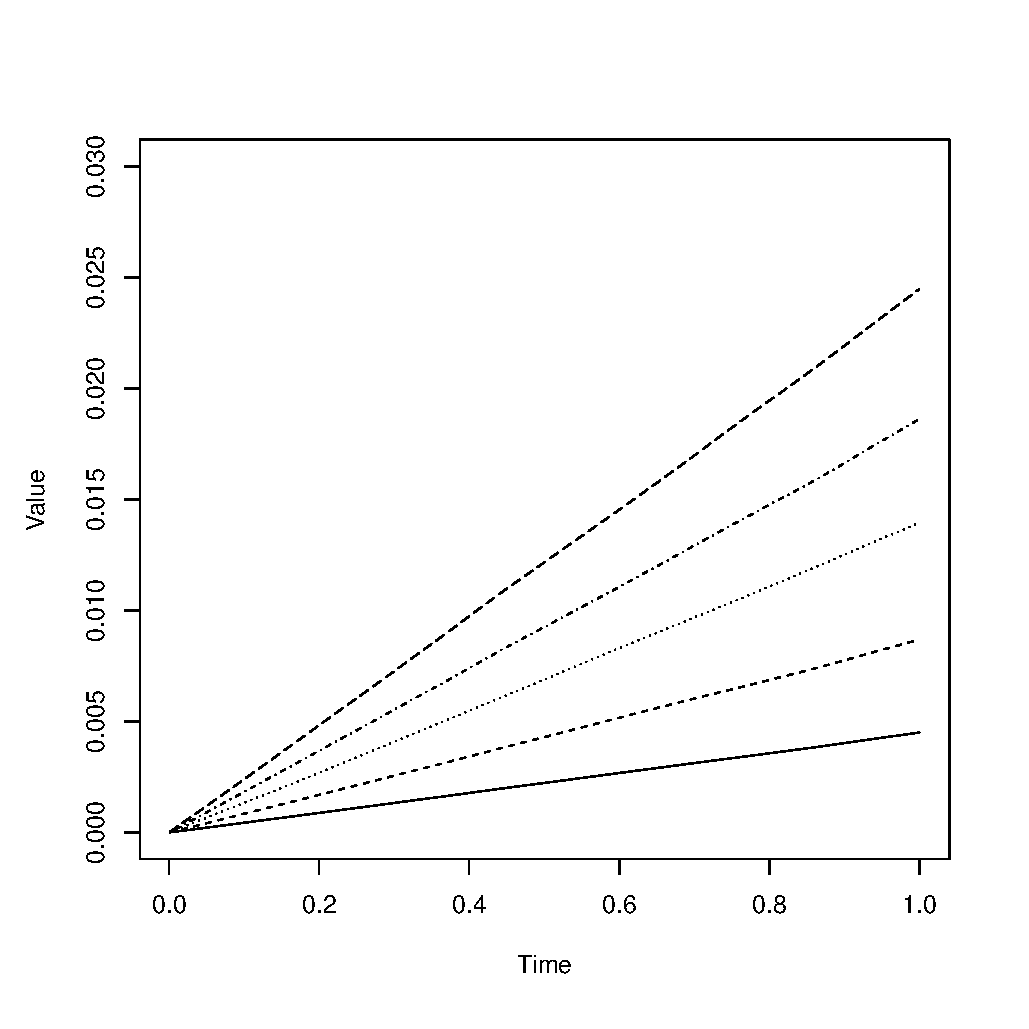
\includegraphics[width=1\textwidth]{StahlPaper2PY}
\caption{Cumulative probability of default \label{fig4}}
\end{minipage}\hfill
\end{framed}
\end{figure}

%\begin{equation}
%d\left[\begin{array}{l} L_1 \\ L_2 \\L_3 \end{array}\right]=
%\left[ \begin{array}{lll} .3 & 0& 0 \\ 0 & .2 & 0 \\ 0 & 0 & .1 \end{array} \right]\left(\left[\begin{array}{c} 1 \\1\\1 \end{array} \right] - \left[\begin{array}{l} L_1 \\ L_2 \\L_3 %\end{array}\right] \right) dt + 
%\left[\begin{array}{ccc} .2 & 0 & 0 \\ .02 & .09797959 & 0 \\ -.09 & .07960842 & .2748863 \end{array}\right]\left[\begin{array}{c} dW_t ^1 \\ dW_t ^2 \\ dW_t ^3\end{array} %\right]
%\end{equation}



\subsection{Total and Marginal Risk}

 For the sake of this example and without loss of generality, it will be assumed that the risk of the portfolio is adequately represented by \(\mathbb{E}[X_T^\lambda]+\sqrt{\mathbb{V}(X_T^\lambda)}\).  The following table summarizes the results.

\begin{table}[H]
\centering
\begin{tabular}{ccccccc}
&\(X_T^1\) & \(X_T^2\)& \(X_T^3\)& \(X_T^4\)& \(X_T^5\)  & Total\\
\hline
p& .005 & .01& .015& .02& .025 & \\
l & 987 &2104 & 1264 & 576 &377 &\\
r & .13 & .15 & .18 & .14 & .78  &\\
\(\rho_j\left(X_T^\lambda\right)\) & 27.62&159.80&103.83&36.08&42.38&369.70 \\
\(\rho_j\left(X_T ^ {\lambda^*}\right)\) & 23.03&170.37&110.02&39.19&27.09&369.70 \\
\(\rho_j(X_T)\) & 20.01&153.34&96.89&32.88&22.01&325.13 \\

\end{tabular}
\end{table}
\(X_T ^ {\lambda^*} \) represents the risk contributions without charging liquidity risk at the loan level: that is, equation (\ref{liquidRiskC}) is used (with \(\lambda_0=\lambda\)) instead of equation (\ref{liquidityRiskContributions}).  \(X_T ^ \lambda\) is superior at charging risk to the loans that truly add more to the riskiness of the portfolio.  The risk of \(X_T ^ 5\) is sharply increased over \(\rho_j (X_T)\) due to its relatively high \(r\), while the risk of \(X_T ^ 2\) barely increases.

%\subsection{Optimization}

\section{Appendix}
\subsection{Expectation of \(z^T Y_T\)}
From equation (\ref{solutionL}) and using the fact that Ito integrals are martingales, 

\begin{equation}
\mathbb{E}[z^T L_T]=z^T \left(\mathbf{1}+e^{-AT}(L_0-\mathbf{1})\right)
\end{equation}
Integrating and using the fact that \(e^A\) is applied component-wise when \(A\) is diagonal,

\begin{equation}
\mathbb{E}[z^T Y_T]=\sum_{i=1} ^ m z_i T+\frac{z_i}{A_{i,i}}\left(1-e^{-{A}_{i, i}T}\right)(L_0^ i-\mathbf{1})\end{equation}

\subsection{Variance of \(z^T Y_T\)}
To find the variance of \(z^T Y_T\) I introduce the following lemma:

\begin{lemma} \label{lemma1}
Let \(I_t\) be a bounded Ito integral  and \(C_t\) be a Riemann integrable function.  Then 
\begin{equation} \label{fubini} \int_ 0^ T  C_t I_t dt=  \int_ 0^ T \left(\int_0 ^ T C_t  dt-\left(\int_0 ^ t C_s ds\right)\right) dI_t
\end{equation}

\end{lemma}

\begin{proof}
By Ito's Lemma,
\begin{equation}
d\left(\int_0 ^ T C_t dt\right) I_T= C_t I_t dt +\left(\int_0 ^ t C_s ds\right) dI_t
\end{equation}
Rearranging and integrating yields equation (\ref{fubini}).
\end{proof}

The only part of equation (\ref{solutionL}) that contributes the variance is the Ito integral.  Hence the problem of finding the variance reduces to 
\begin{equation}
\mathbb{V}(z^T Y_T)=\mathbb{V}\left(z^T \int_0 ^ T e^{-At} \int_ 0 ^ t e^{As} \Sigma dW_s dt \right)
\end{equation}

Letting \(C_t=e^{-At}\) and \(I_t=\int_ 0 ^ t e^{As} \Sigma dW_s \) and using lemma \ref{lemma1},

\begin{equation}
=\mathbb{V}\left(z^T  \int_ 0 ^ T \frac{1}{A}\left( e^{-At} -e^{-AT} \right) e^{At}\Sigma dW_t  \right)
\end{equation}
Where \(\frac{1}{A}\) is defined as component-wise division and \(\mathbf{I}\) is the identity matrix.

\begin{equation}
=\mathbb{V}\left(z^T  \int_ 0 ^ T \frac{1}{A}\left( \mathbf{I}-e^{-A(T-t)} \right)\Sigma dW_t  \right)
\end{equation}

\begin{equation}
=\int_ 0 ^ T z^T M_t \Sigma \Sigma ^T M_t^T z dt  
\end{equation}
Where \(M_t=\frac{1}{A}\left( \mathbf{I}-e^{-A(T-t)} \right)\).

\begin{equation}
=\int_0 ^ T \sum_{i=1} ^ m \sum_{j=1} ^ m z_i z_j \sigma_i \sigma_j \rho_{i,j} \frac{1}{A_{i,i}}\left(1-e^{-{A}_{i, i}(T-t)}\right)\frac{1}{A_{j,j}}\left(1-e^{-{A}_{j, j}(T-t)}\right) dt\end{equation}

Integrating yields equation (\ref{varianceY}).
\subsection{Expectation of \(X_T\)}

\begin{equation}
\mathbb{E}[X_T]=\frac{\partial \phi_{X_T}}{\partial u} \big|_{u=0}
\end{equation}

\begin{equation}
 =\frac{\partial e^{\mu(z)+\frac{\sigma^2(z)}{2} }}{\partial u} \bigg|_{u=0}\end{equation}
 
 \begin{equation}
 = e^{\mu(z)+\frac{\sigma^2(z)}{2} } \left(\mu(z')+\frac{1}{2} \sigma^2 (z', \mathbf{1})\right) \bigg|_{u=0}\end{equation}
 
 \begin{equation}
 =\mu(d)
 \end{equation}
 Where \(d=z'=\frac{1}{i}\sum_j p_j \phi_j'(0) w_{j, k} \)
 
 \subsection{Variance of \(X_T\)}
 
\begin{equation}
\mathbb{V}(X_T)=\frac{\partial^2 \phi_{X_T}}{\partial u^2} \big|_{u=0}
\end{equation}

\begin{equation}
 =\frac{\partial ^2 e^{\mu(z)+\frac{\sigma^2(z)}{2} }}{\partial u^2} \bigg|_{u=0}\end{equation}
 
 \begin{equation}
 = e^{\mu(z)+\frac{\sigma^2(z)}{2} } \left(\mu(z'')+ \sigma^2 (z') \right) \bigg|_{u=0}\end{equation}
 
 \begin{equation}
 =\mu(d^2)+\sigma^2 (d)
 \end{equation}
 Where \(d^2=z''=-\sum_j p_j \phi_j''(0) w_{j, k} \)
 
 \subsection{Expectation of \(X_T ^ \lambda \)}
 \begin{equation}
 \mathbb{E}[X_T ^ \lambda]=\frac{\partial \phi_{X_T ^\lambda}(u^\lambda)}{\partial u} \big|_{u=0}
 \end{equation}
 
 \begin{equation}
 \mathbb{E}[X_T ^ \lambda]=\mathbb{E}[X_T](1+q\lambda)
 \end{equation}
 
  \subsection{Variance of \(X_T ^ \lambda \)}
 \begin{equation}
 \mathbb{V}(X_T ^ \lambda)=\frac{\partial^2 \phi_{X_T ^\lambda}(u^\lambda)}{\partial u^2} \big|_{u=0}
 \end{equation}
 
 \begin{equation}
 \mathbb{V}(X_T ^ \lambda)=\mathbb{E}[X_T](1+q\lambda)
 \end{equation}
\\
\\
%The key takeaway is that \emph{no  optimization must be done}.  The economic capital must be pushed down to the individual loan officers and by tying this capital to their compensation they will automatically choose an optimal allocation of loans.  

%\section{Expected Value [no liquidity]}
%Letting \(d\) be the vector \(d=\sum_j p_j l_j w_{j, k}\), 
%\[\mathbb{E}[X]=\mu(d) \]

%\section{Variance[No liquidity]}
%Letting \(d ^2\) be the vector \(d^2=\sum_j p_j l_j^2 w_{j, k}\),
%\[\mathbb{V}(X)=\mu(d ^2)+\sigma^2(d)\]


Duffie, D., Pan, J., Singleton, K., 2000. Transform analysis and asset pricing for affine jump diffusions.
Econometrica 68, 1343–1376.

Filipovic, D., 2001. A general characterization of one factor affine term structure models. Finance and !
Stochastics 5, 389–412.
\end{document}
